\chapter{Módulo: Clientes}
\label{mod:06-clientes}

\section{Propósito}
\label{sec:clientes-proposito}

Gestiona el ABM de clientes de venta --- distintos de los pacientes clínicos, aunque pueden ser la misma persona física --- con sus datos de facturación (persona física o jurídica). Es el módulo que le da a \code{Venta} a quién facturarle.

\section{Entidades principales}
\label{sec:clientes-entidades}

\begin{longtable}{p{2.8cm}p{10.5cm}}
\caption{Entidades principales del módulo de Clientes.}\label{tab:clientes-entidades}\\
\toprule
\textbf{Entidad} & \textbf{Rol} \\
\midrule
\endfirsthead
\toprule
\textbf{Entidad} & \textbf{Rol} \\
\midrule
\endhead
\bottomrule
\endfoot
\code{Cliente} & Identidad de facturación de una \code{Person}: tipo (física/jurídica), razón social, RUC/CI fiscal, contacto. Ver Capítulo~\ref{sec:modelo-datos}, Grupo A. \\
\end{longtable}

\section{Reglas de negocio clave}
\label{sec:clientes-reglas}

\begin{itemize}
  \item \textbf{\code{Cliente} siempre cuelga de \code{Person}} (FK único \code{PersonId}) --- no es una entidad de facturación separada. \code{TipoFacturacion} más \code{RazonSocial} más \code{RucCiFiscal} más \code{Direccion}/\code{Email}/\code{Telefono} son simplemente el dato de facturación de esa persona \emph{en su rol de cliente}. Ver \hyperref[adr:0001]{ADR 0001 --- Person como raíz de identidad}.
  \item \textbf{\code{Cliente} y \code{Patient} pueden compartir la misma \code{Person}} sin relación directa entre ellos --- se relacionan únicamente a través de \code{Person} (no hay FK \code{Cliente}$\leftrightarrow$\code{Patient}). Un paciente que además compra productos no genera una persona duplicada.
  \item \textbf{Alta por reutilización de \code{Person}:} \code{GET /api/clientes/}\allowbreak \code{buscar-persona?ci=} busca si ya existe una \code{Person} con esa CI; si existe, se reutiliza (evita duplicar datos si la persona ya es paciente); si no, se crea una nueva junto con el \code{Cliente}.
  \item \textbf{No hay borrado físico simple:} \code{DELETE /api/clientes/{id}} desactiva (soft delete); reactivar es \code{POST /api/clientes/{id}/activar}. En el frontend, ambas acciones viven exclusivamente en el menú contextual de la tabla (modales de confirmación verde/rojo), nunca en el formulario de edición.
  \item \textbf{\code{Venta.ClienteId} es nullable} --- \code{null} significa ``Consumidor Final'', una venta no exige tener un cliente registrado.
  \item \textbf{Origen histórico:} hasta la migración \code{035_Clientes}, los datos de facturación colgaban 1:1 de \code{Patient} (\code{DatosFacturacion}, hoy eliminada); esa migración copió los datos existentes hacia \code{Cliente} (mapeando \code{PatientId}$\to$\code{PersonId}) y dropeó la tabla vieja.
\end{itemize}

\section{Endpoints}
\label{sec:clientes-endpoints}

Detalle completo (policies, DTOs) en el Apéndice de Referencia de API, \S 2.\ Personas (\code{Clientes}\allowbreak \code{Controller}).

\begin{longtable}{p{3.4cm}p{4.0cm}p{5.9cm}}
\caption{Endpoints principales del módulo de Clientes.}\label{tab:clientes-endpoints}\\
\toprule
\textbf{Método} & \textbf{Ruta} & \textbf{Descripción} \\
\midrule
\endfirsthead
\toprule
\textbf{Método} & \textbf{Ruta} & \textbf{Descripción} \\
\midrule
\endhead
\bottomrule
\endfoot
GET & \code{/api/clientes} & Listado paginado (filtros: búsqueda, estado, tipo) \\
GET & \code{/api/clientes/{id}} & Detalle \\
GET & \code{/}\allowbreak \code{api/}\allowbreak \code{clientes/}\allowbreak \code{buscar-persona?ci=} & Busca \code{Person} existente por CI, para reutilizar al dar de alta \\
POST & \code{/api/clientes} & Alta \\
PUT & \code{/api/clientes/{id}} & Edición \\
DELETE $\cdot$ POST & \code{/api/clientes/{id}} $\cdot$ \code{/{id}/activar} & Desactivar / reactivar \\
\end{longtable}

\section{Flujo típico}
\label{sec:clientes-flujo}

Alta de cliente durante el armado de una venta (el caso de uso más frecuente en la práctica, más que el ABM directo):

\begin{figure}[htbp]
\centering
\begin{tikzpicture}
  \node[actor] (u) at (0,0) {Recepción\\\footnotesize VentaEditor};
  \node[actor] (sel) at (3.6,0) {ClienteSelector};
  \node[actor] (modal) at (7.2,0) {ClienteQuick-\\CreateModal};
  \node[actor] (api) at (10.8,0) {ClientesController};

  \draw[lineavida] (u.south) -- ++(0,-5.8);
  \draw[lineavida] (sel.south) -- ++(0,-5.8);
  \draw[lineavida] (modal.south) -- ++(0,-5.8);
  \draw[lineavida] (api.south) -- ++(0,-5.8);

  \draw[mensaje] ($(u.south)+(0,-0.8)$) -- node[above,font=\scriptsize]{busca cliente por nombre/CI} ($(sel.south)+(0,-0.8)$);

  \node[font=\scriptsize\itshape] at (0,-1.6) {si no existe:};
  \draw[mensaje] ($(u.south)+(0,-2.2)$) -- node[above,font=\scriptsize,align=center]{``Nuevo cliente''\\(permiso crear\_cliente)} ($(sel.south)+(0,-2.2)$);
  \draw[mensaje] ($(sel.south)+(0,-3.0)$) -- node[above,font=\scriptsize]{abre modal} ($(modal.south)+(0,-3.0)$);
  \draw[mensaje] ($(u.south)+(0,-3.8)$) -- node[above,font=\scriptsize,align=center]{elige modo: paciente activo\\existente $\vert$ persona nueva} ($(modal.south)+(0,-3.8)$);
  \draw[mensaje] ($(modal.south)+(0,-4.6)$) -- node[above,font=\scriptsize]{GET /clientes/buscar-persona?ci= (si aplica)} ($(api.south)+(0,-4.6)$);
  \draw[mensaje] ($(modal.south)+(0,-5.2)$) -- node[above,font=\scriptsize]{POST /clientes} ($(api.south)+(0,-5.2)$);
  \draw[mensajeretorno] ($(sel.south)+(0,-5.7)$) -- node[below,font=\scriptsize]{cliente creado, queda seleccionado} ($(api.south)+(0,-5.7)$);
\end{tikzpicture}
\caption{Alta rápida de cliente embebida en el armado de una venta: si el cliente no existe, se busca primero una \texttt{Person} existente por CI antes de crear una nueva.}
\label{fig:seq-alta-cliente}
\end{figure}

Si el cliente ya existe, \code{ClienteSelector} simplemente lo deja seleccionado sin pasar por el modal.

\section{Vistas de frontend}
\label{sec:clientes-vistas}

\begin{itemize}
  \item \code{ClientesView.vue} --- ABM principal (listado, alta/edición, activar/desactivar por menú contextual).
  \item \code{ClienteSelector.}\allowbreak \code{vue} (componente, no vista) --- buscador de clientes activos más opción ``Consumidor Final'' más botón ``Nuevo cliente'', usado embebido en los editores de venta/presupuesto.
  \item \code{ClienteQuickCreateModal.}\allowbreak \code{vue} (componente) --- alta rápida en dos modos (paciente activo existente / persona nueva) con datos de facturación, invocado desde \code{ClienteSelector}.
\end{itemize}

\section{Interfaz}
\label{sec:clientes-interfaz}

\begin{figure}[htbp]
\centering
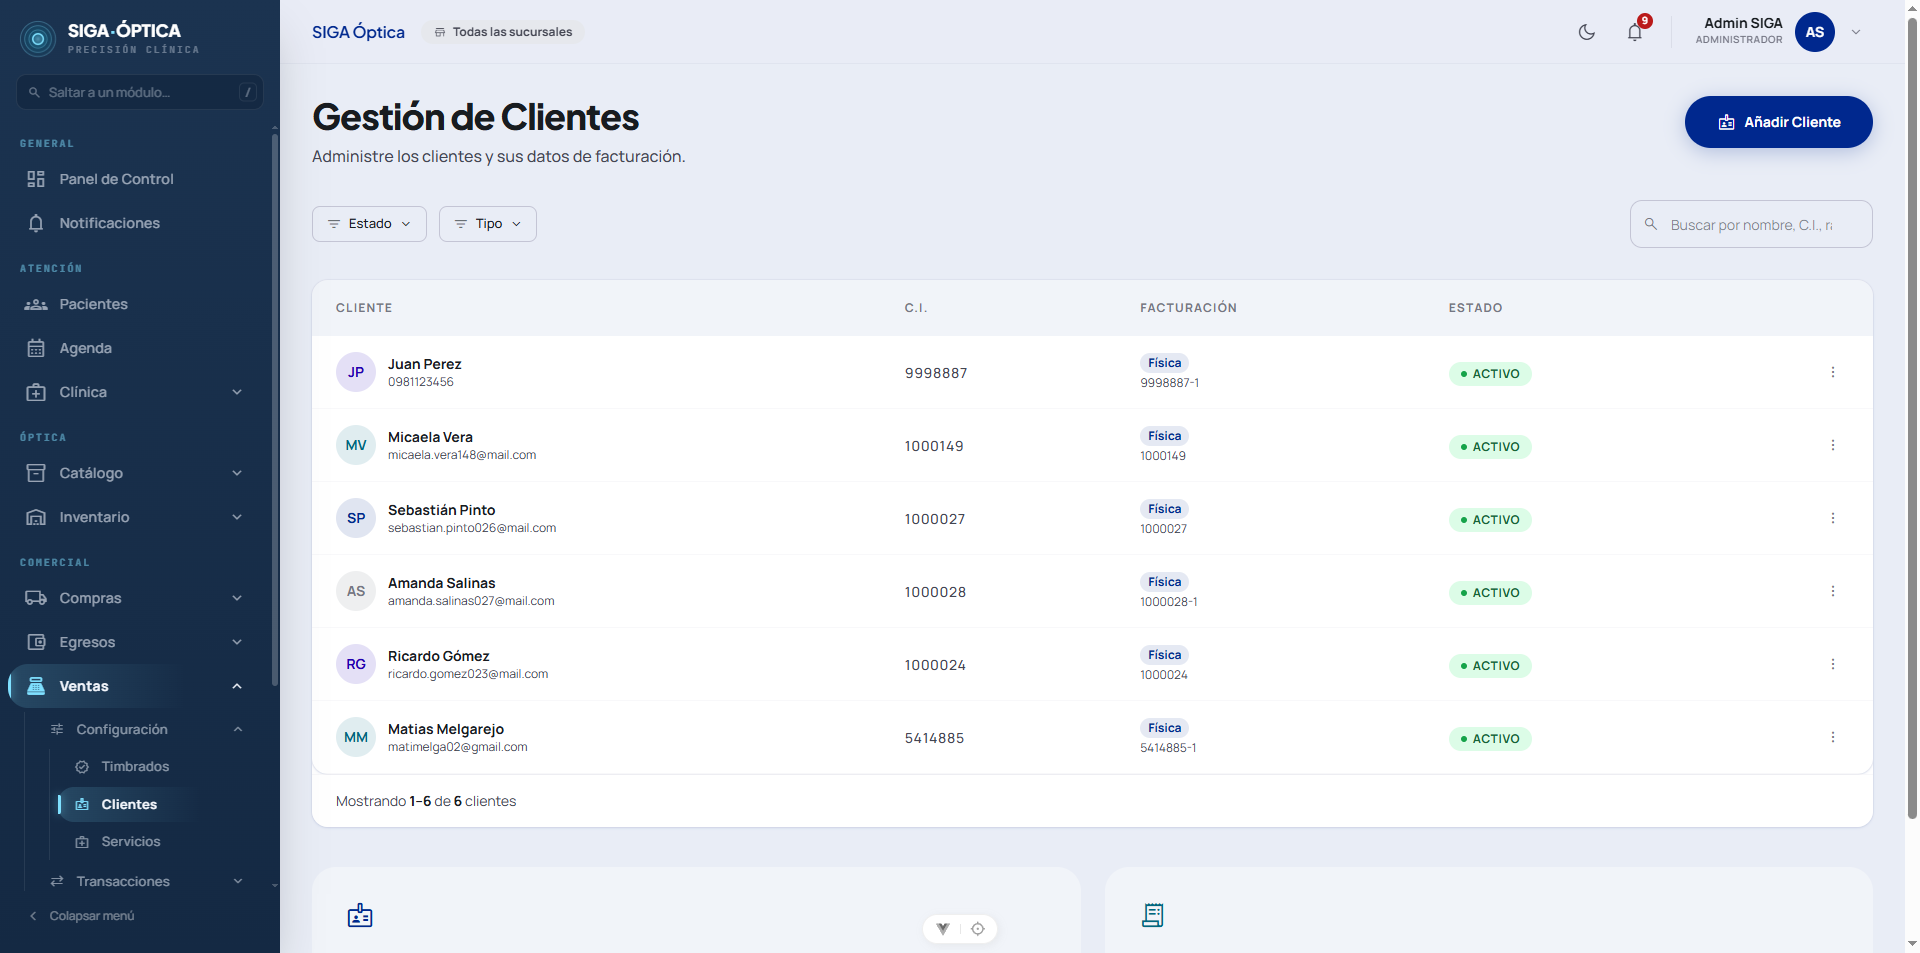
\includegraphics[width=0.95\textwidth]{imagenes/mod06-clientes.png}
\caption{Gestión de clientes, con su tipo de facturación y estado.}
\label{fig:mod06-clientes}
\end{figure}

\section{Estado}
\label{sec:clientes-estado}

\Implementado, integrado con Ventas (\code{Venta.ClienteId} reemplazó a la referencia previa por \code{PatientId}). \code{ventasService} y todas las vistas de venta/presupuesto/trabajo muestran \code{clienteNombre}, con fallback a ``Consumidor Final''.
